\documentclass{beamer}

% Beamer style
% Beamer style
%\usetheme[secheader]{Madrid}
% \usetheme{CambridgeUS}
\useoutertheme{infolines}
\usecolortheme[rgb={0.65,0.15,0.25}]{structure}
% \usefonttheme[onlymath]{serif}
\beamertemplatenavigationsymbolsempty
%\AtBeginSubsection


% Packages
\usepackage[latin1]{inputenc}
\usepackage{color}
\usepackage{amsmath, amsfonts, amssymb}
\usepackage{marvosym}
\usepackage{graphicx}
\usepackage{/home/robin/LATEX/Biblio/astats}

% Commands
\definecolor{darkred}{rgb}{0.65,0.15,0.25}
\definecolor{darkgreen}{rgb}{0,0.4,0}
%\newcommand{\emphase}[1]{\textcolor{darkred}{#1}}
\newcommand{\Esp}{\mathbb{E}}
\newcommand{\dd}{\text{d}}
\newcommand{\emphase}[1]{{#1}}
\newcommand{\paragraph}[1]{\textcolor{darkred}{#1}}
\newcommand{\refer}[1]{\textcolor{gray}{\footnotesize{[\cite{#1}]}}}
\newcommand{\Refer}[1]{\textcolor{gray}{\footnotesize{[#1]}}}
\newcommand{\ra}{$\emphase{\rightarrow} \;$}

% Names
\newcommand{\chr}{}
\newcommand{\comment}{}

%====================================================================
\title[Genomic alterations]{Looking for recurrent genomic alterations: \\ A race with technologies}

\author[S. Robin]{S. Robin}

\institute[AgroParisTech / INRA]{
  \bigskip
 \begin{tabular}{ccccc}
    
\includegraphics[width=.15\textwidth]{../FIGURES/LogoINRA-Couleur} & 
    \hspace{.02\textwidth} &
    
\includegraphics[width=.225\textwidth]{../FIGURES/logagroptechsolo} & 
    \hspace{.02\textwidth} &
    
\includegraphics[width=.15\textwidth]{../FIGURES/logo-ssb} \\ 
  \end{tabular} \\
  \bigskip
  {
    \begin{tabular}{rll}
    Joint work with & V. Stefanov;  \\
    On-going work with & L. Decreusefond, M.-P. Etienne, G. Lang, P. Vallois. 
    \end{tabular} ~\\ ~\\ ~\\
    }
  }

  \date[Montpellier, 2015]{S�minaire I3M, Montpellier, October 2014}

%====================================================================

%====================================================================
%====================================================================
\begin{document}
%====================================================================
%====================================================================

%====================================================================
\frame{\titlepage
  }
  
%====================================================================
\section*{Genomic alterations}
\frame{\frametitle{Genomic alterations}}
  
%====================================================================
\frame{\frametitle{Genomic alterations in cancer cells}

  $$
  \begin{tabular}{cc}
    \onslide+<1->{Normal cell} & \onslide+<2->{Tumor cell} \\
    \onslide+<1->{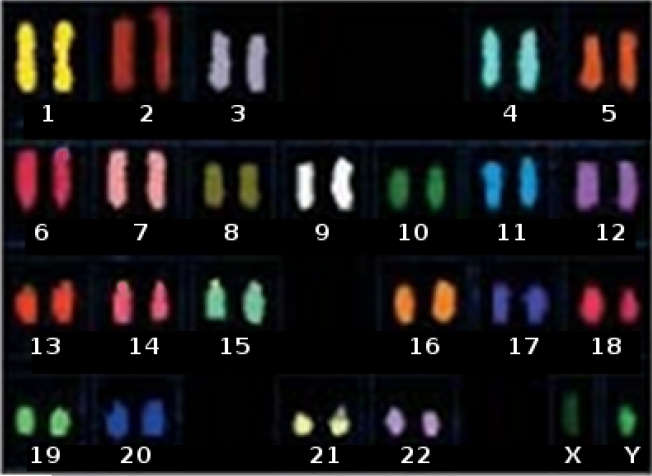
\includegraphics[height=.4\textheight]{../FIGURES/Hup08-Fig121b}}
    &
    \onslide+<2->{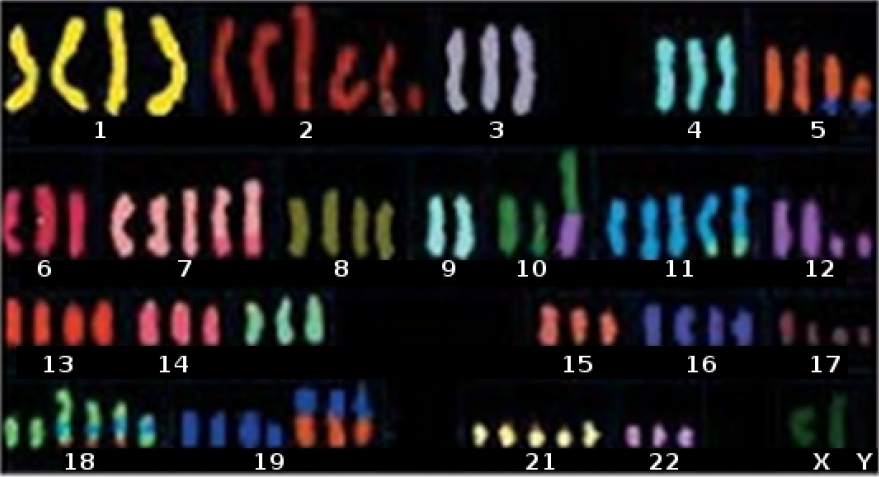
\includegraphics[height=.4\textheight]{../FIGURES/Hup08-Fig121a}}
  \end{tabular}
  $$
  \onslide+<2->{
  \refer{Hup08}
  }
}

%====================================================================
\frame{\frametitle{Detection of the alterations}

  $$
  \begin{tabular}{cc}
    Karyotype & {CGH profile}  \\
	 \\
    \begin{tabular}{l}
    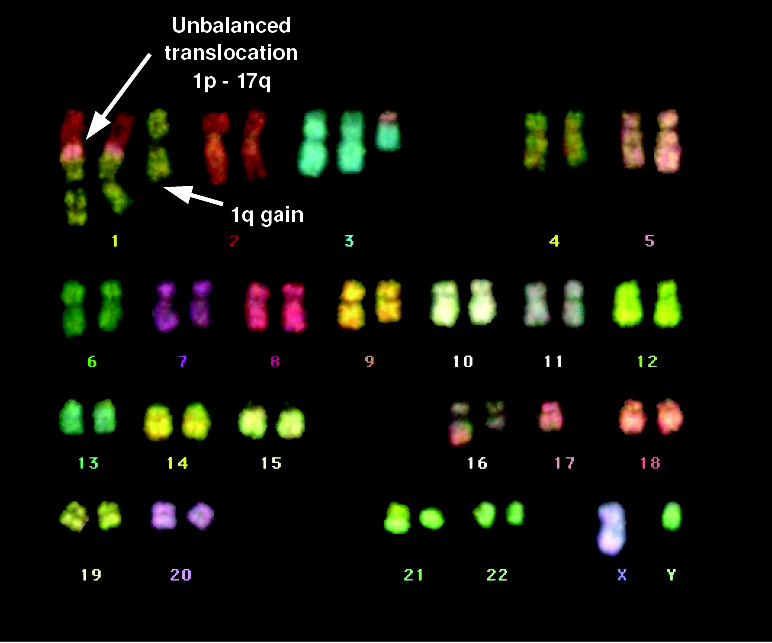
\includegraphics[height=.43\textheight]{../FIGURES/Hup08-Fig128b}
    \end{tabular}
    &
    \begin{tabular}{l}
    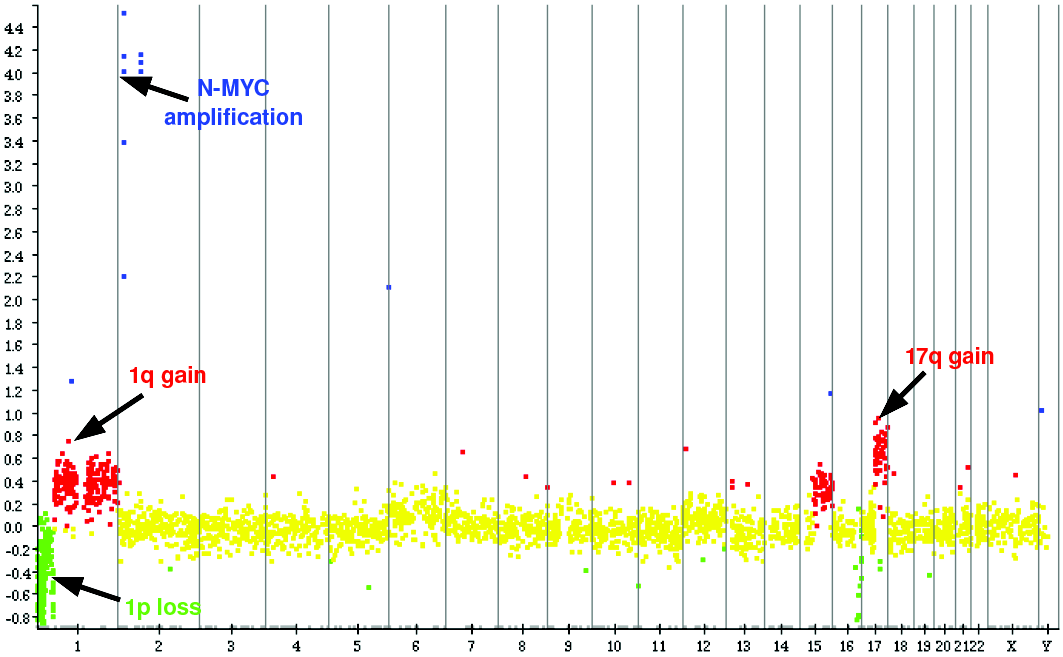
\includegraphics[height=.43\textheight]{../FIGURES/Hup08-Fig128a}
    \end{tabular}
  \end{tabular}
  $$
  \refer{Hup08}. 

}

%====================================================================
\frame{\frametitle{Recurrent alterations}

  \vspace{-.05\textheight}
  $$
  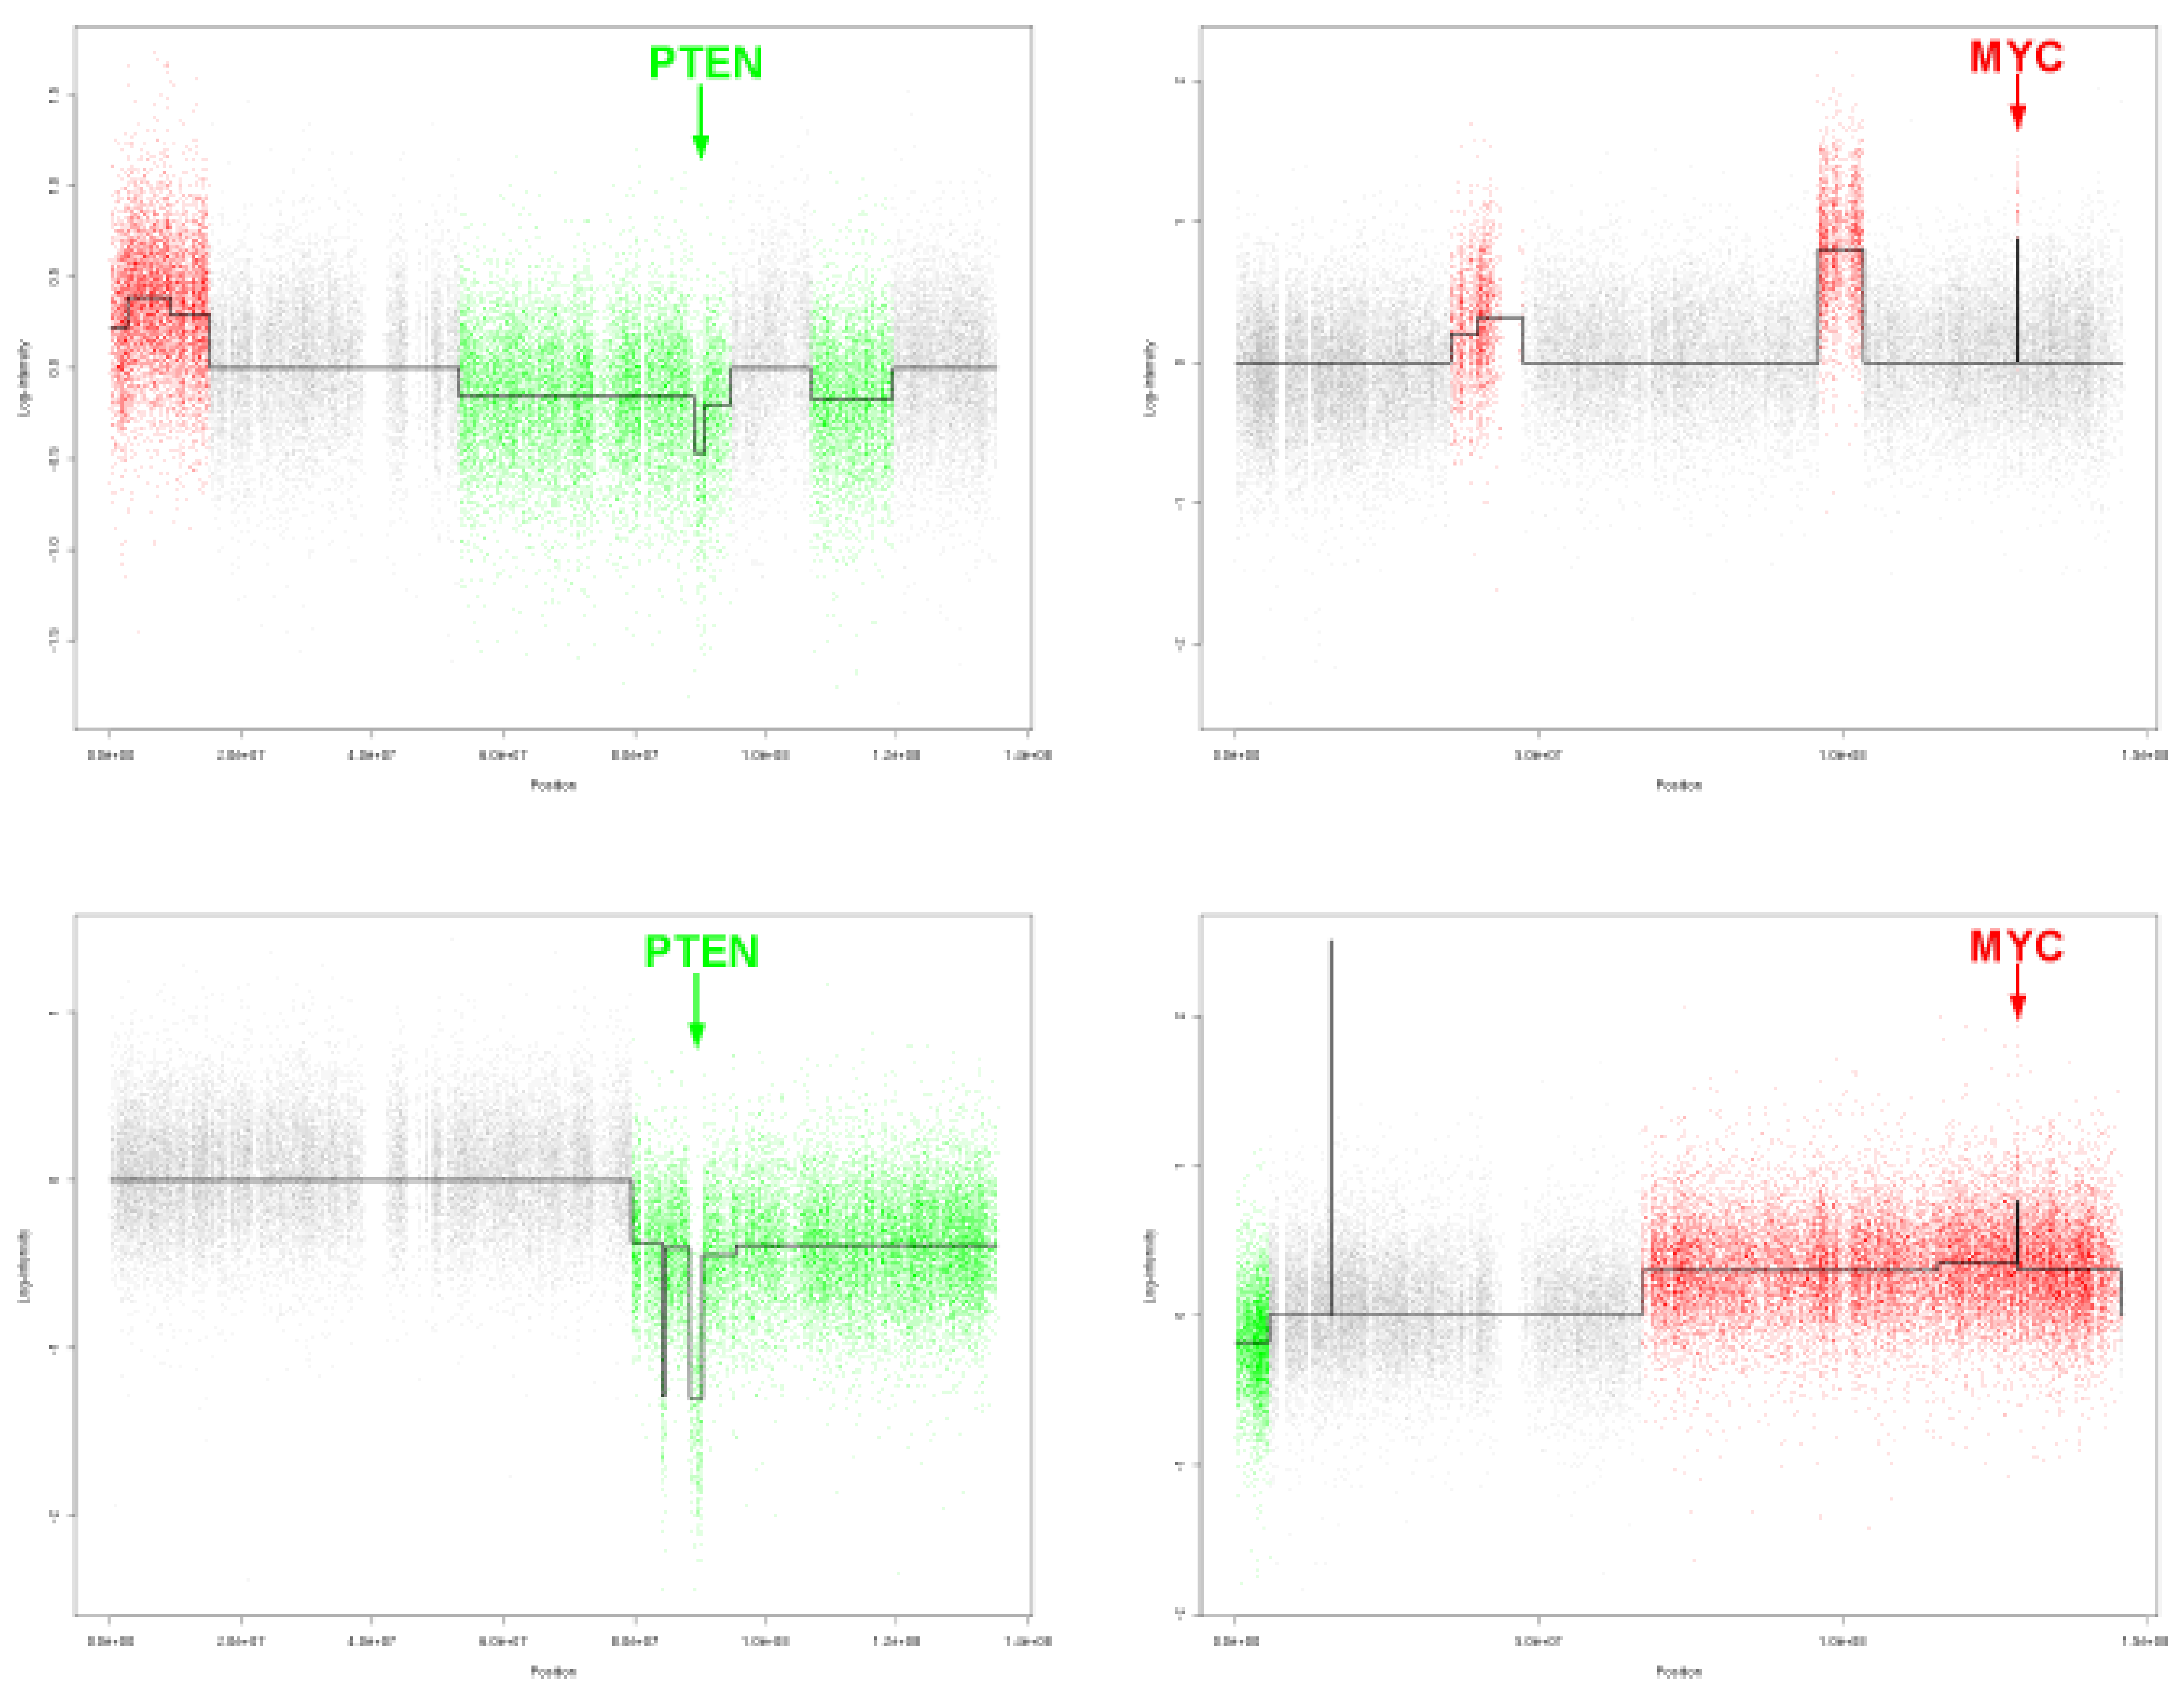
\includegraphics[height=.8\textheight]{../FIGURES/Rig10-Fig6-5}
  $$
  Chrom. 10 and 8 of two patients with breast carcinomas. \refer{Rig11} 
}

%====================================================================
\frame{\frametitle{Profiles}

  \begin{tabular}{cc}
    \begin{tabular}{p{0.5\textwidth}}
    \onslide+<1->{\paragraph{Individual profiles:} 
    patient $i$, locus $t$, 
    $$
    X_i(t) = \left\{
	 \begin{array}{ll}
	 0 & \text{if normal} \\
	 1 & \text{if \textcolor{red}{altered}}
	 \end{array}
    \right.
    $$
   }
    \onslide+<2->{\paragraph{Cumulated profile:}
    $$
    S_p(t) = \sum_{i=1}^p X_i(t)
    $$
    $= $ nb of altered patients at locus $t$ \\
   }
    \onslide+<3->{\bigskip
    \paragraph{Significance:}}
    \end{tabular}
    &
    \hspace{-0.1\textwidth}
    \begin{tabular}{c}
	 \begin{overprint}   
%	 \onslide<1>    
%	 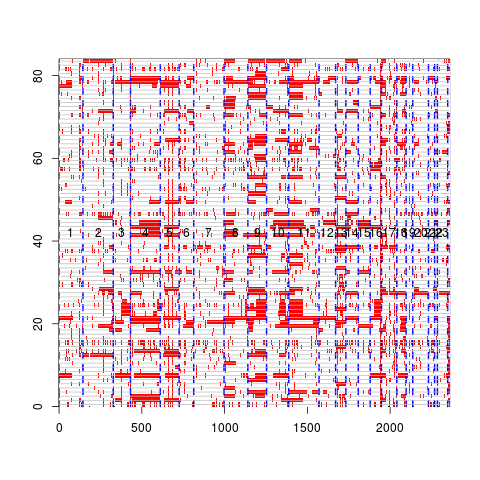
\includegraphics[height=.7\textheight, width=.5\textwidth]{../FIGURES/Fig-MinReg-Data-Prof} 
% 	 \onslide<2>    
% 	 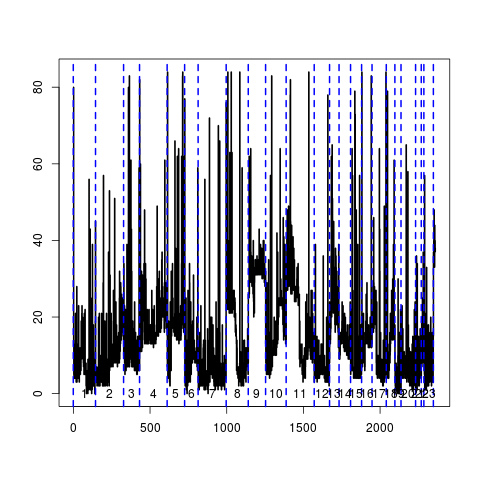
\includegraphics[height=.7\textheight, width=.5\textwidth]{../FIGURES/Fig-MinReg-Data-Cumul} 
	 \onslide<1>    
	 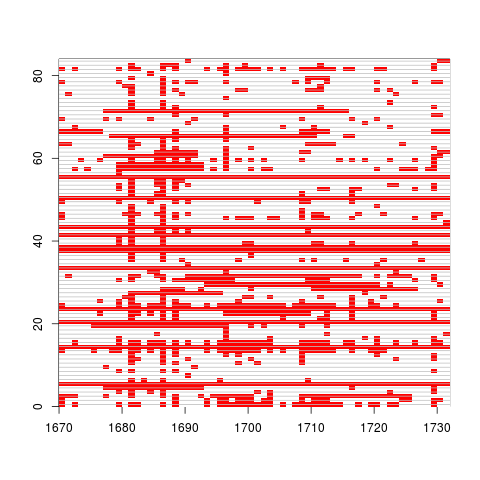
\includegraphics[height=.7\textheight, width=.5\textwidth]{../FIGURES/Fig-MinReg-Data-Prof13} 
	 \onslide<2>    
	 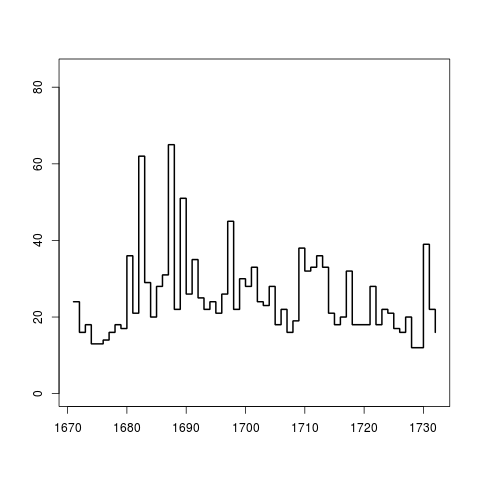
\includegraphics[height=.7\textheight, width=.5\textwidth]{../FIGURES/Fig-MinReg-Data-Cumul13} 
	 \onslide<3>    
	 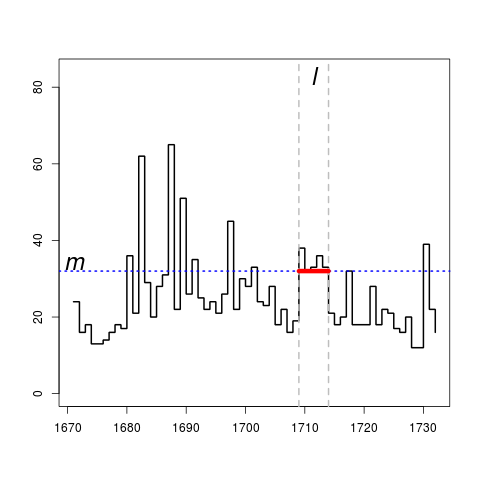
\includegraphics[height=.7\textheight, width=.5\textwidth]{../FIGURES/Fig-MinReg-Data-Reg1-13} 
	 \onslide<4>    
	 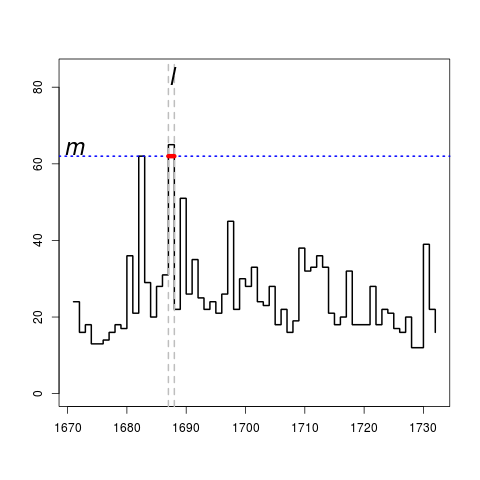
\includegraphics[height=.7\textheight, width=.5\textwidth]{../FIGURES/Fig-MinReg-Data-Reg2-13} 
	 \end{overprint}   
    \end{tabular}
  \end{tabular}
  \onslide+<3->{
  $$
  \pi(m, \ell) = \Pr\left\{\text{
  an excursion with length $\ell$ above level $m$ occurs
  }\right\}
  $$}

  }


%====================================================================
\frame{\frametitle{Abacus}

  \paragraph{Significance isolines:} for given cohort size $p$, number of loci $n$ and parameter $\theta \approx $ (mean nb. alterations, mean alteration length)
  $$
  \mathcal{C}_\alpha(\theta) = \{(m, \ell): \pi(m, \ell) = \alpha\}
  $$
  (e.g. $\alpha = 1\%$) \vspace{-.1\textheight}
  $$
  \begin{array}{rc}
    \begin{array}{c} \rotatebox{90}{threshold $m$} \end{array} & 
    \begin{array}{c} 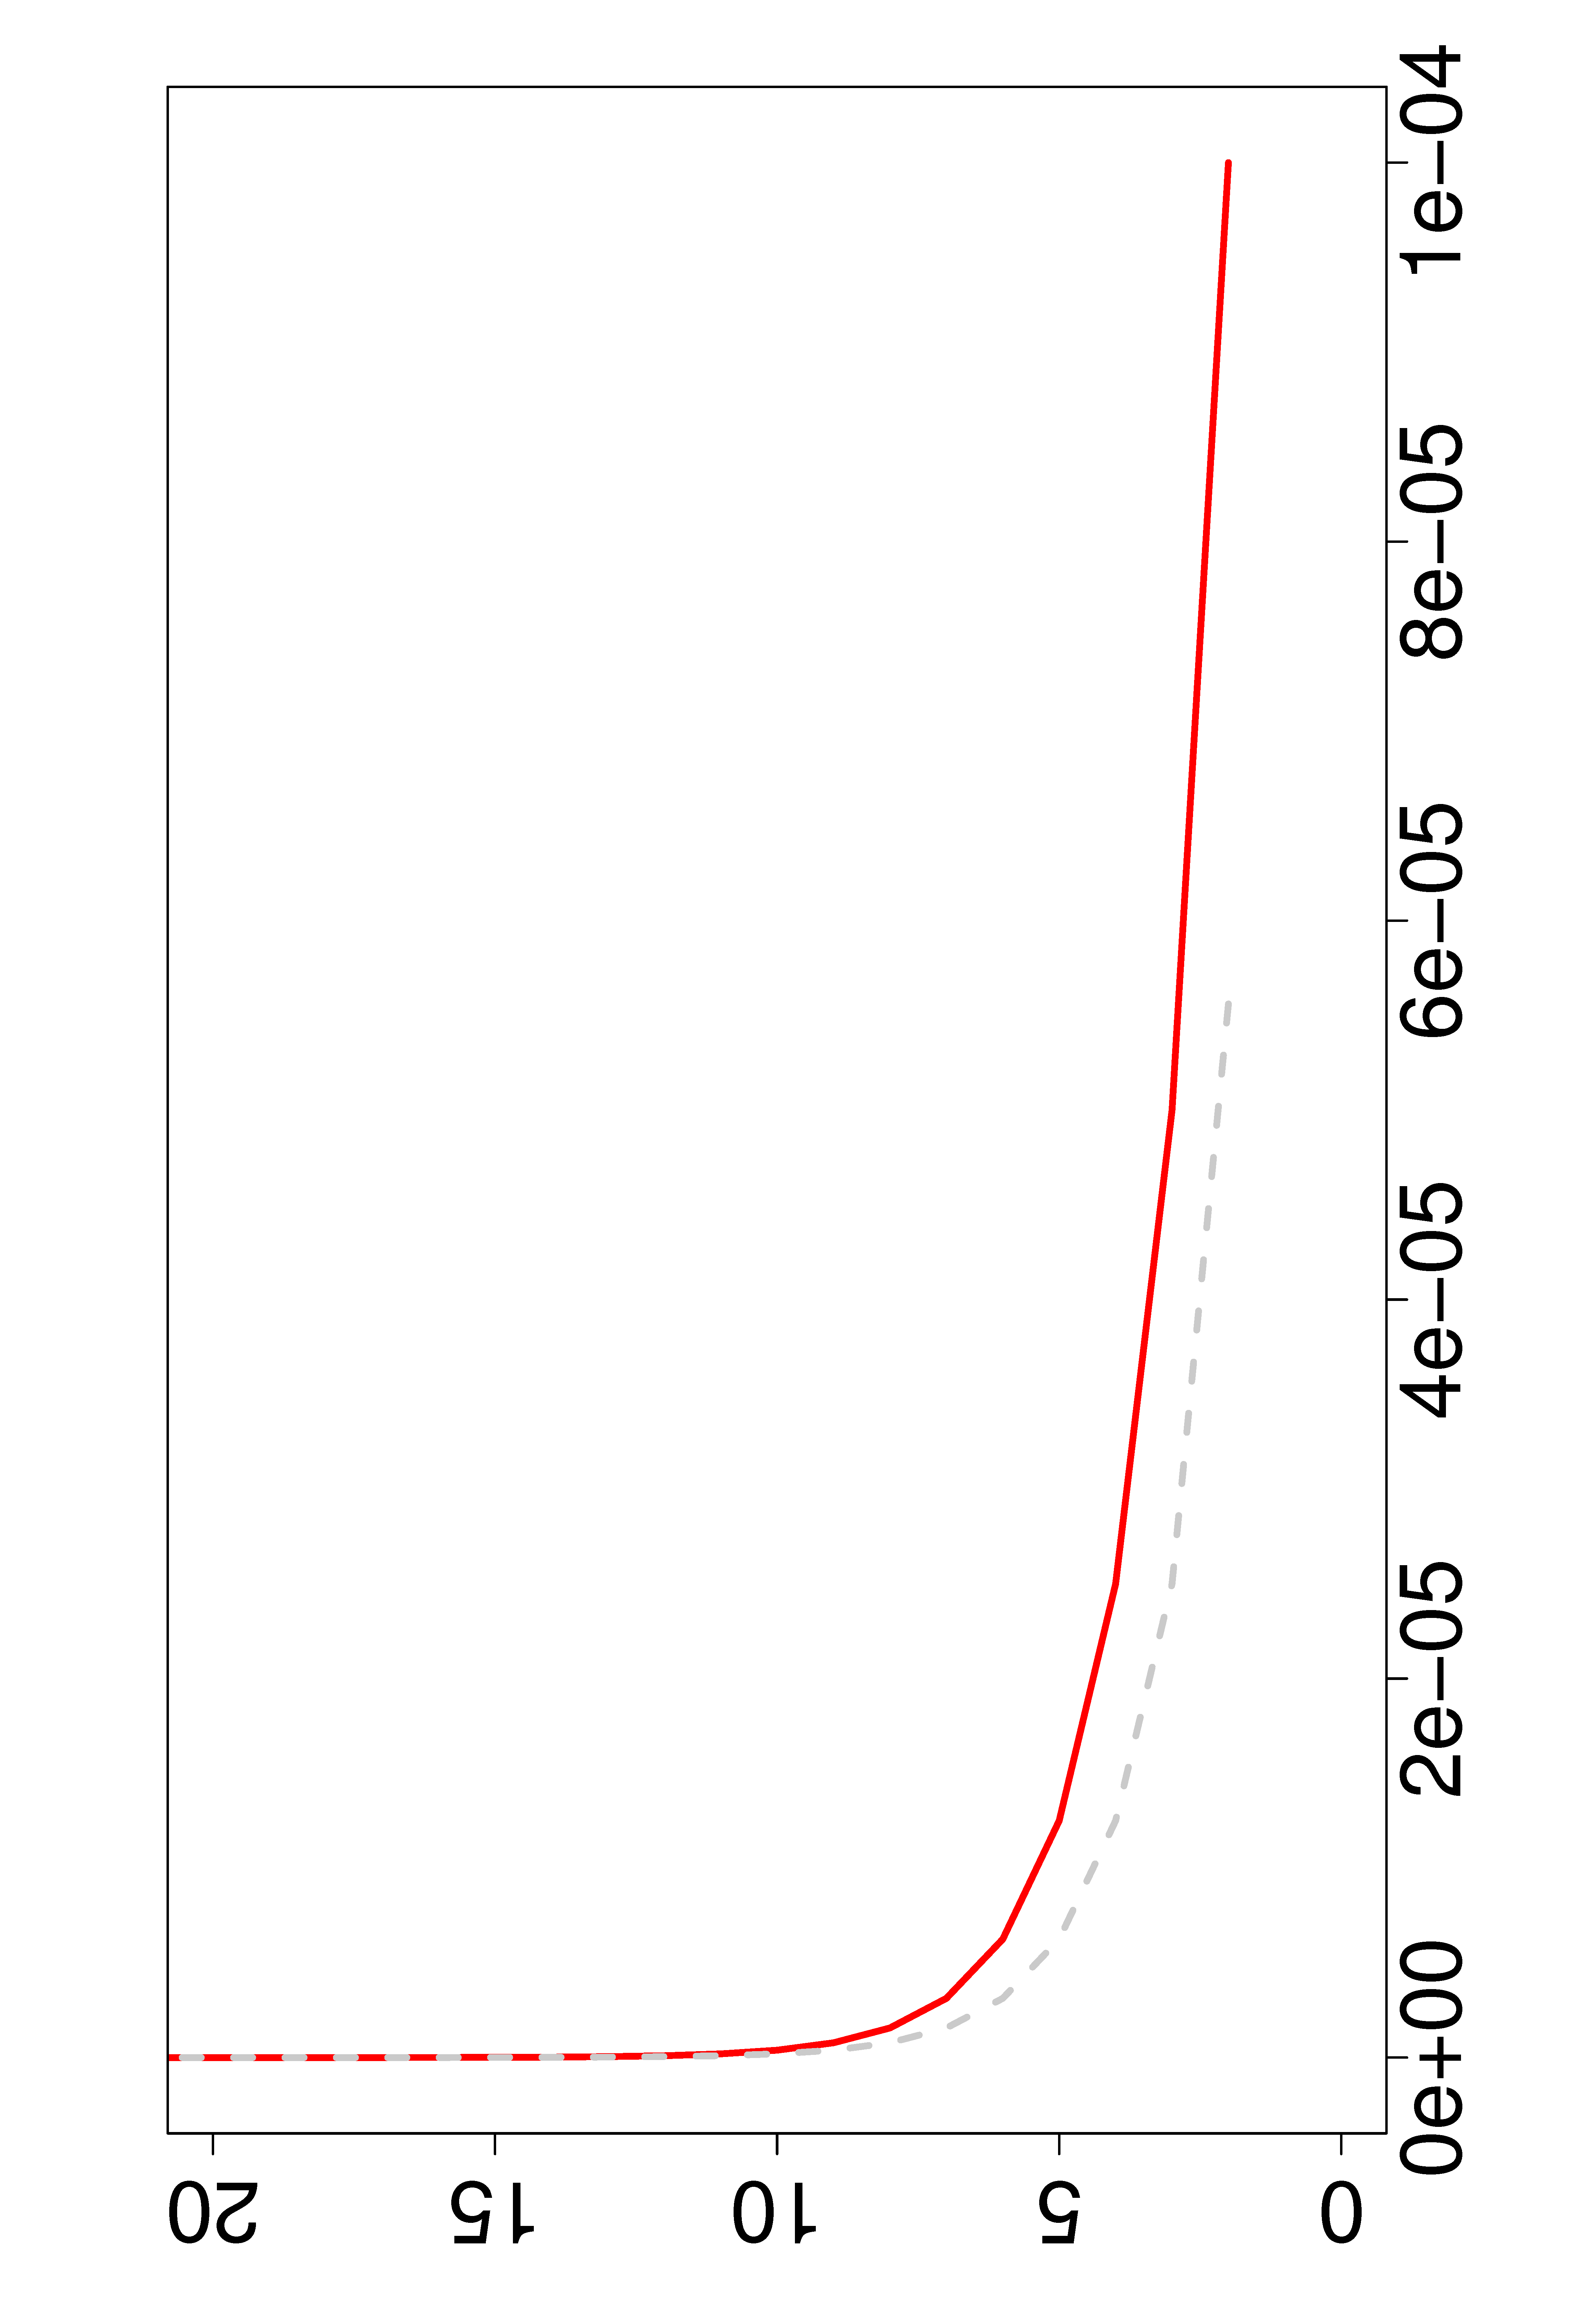
\includegraphics[height=.7\textheight, width=.45\textwidth, angle=270]{../FIGURES/Abaque-Example} \end{array} \\
    & \text{relative alteration length } \ell / n
  \end{array}
  $$
}

%====================================================================
\frame{\frametitle{Outline}
  \tableofcontents
}

%====================================================================
\section{Few loci, few patients}
\frame{\frametitle{Few loci, few patients}}
  
%====================================================================
\section{Many loci, few patients}
\frame{\frametitle{Many loci, few patients}}
  
%====================================================================
\section{Many loci, many patients}
\frame{\frametitle{Many loci, many patients}}
  
%====================================================================
{\tiny
  \bibliographystyle{/home/robin/LATEX/Biblio/astats}
  \bibliography{/home/robin/Biblio/AST,/home/robin/Biblio/ARC,/home/robin/Biblio/SSB}
  }

%====================================================================
%====================================================================
\end{document}
%====================================================================
%====================================================================
